\documentclass[a4paper,12pt]{article}
\usepackage{graphicx}
\usepackage{amsmath}
\usepackage{geometry}
\usepackage{float}
\usepackage{tikz}
\usepackage{booktabs}
\usepackage{algorithm}
\usepackage{algorithmic}
\usepackage{array}
\usepackage{hyperref}
\usepackage{listings}
\usepackage{xcolor}
\usetikzlibrary{shapes.geometric, arrows, positioning, calc}

\geometry{margin=1in}

\title{Scientific Calculator Using AVR-GCC}
\author{EE24BTECH11002 - Agamjot Singh}
\date{\today}

\begin{document}

\maketitle

\section{Shunting Yard Algorithm Algorithm Overview}

The Shunting Yard algorithm uses two main data structures:
\begin{itemize}
    \item A stack for temporarily storing operators
    \item An output queue for the final postfix expression
\end{itemize}

The algorithm processes each token in the input expression sequentially, following specific rules based on the token type[3].

\subsection{Key Terms}

\begin{itemize}
    \item \textbf{Token}: A number, operator, function, or parenthesis in the expression
    \item \textbf{Operator}: Mathematical symbols representing operations $(+, -, *, /, \vee)$
    \item \textbf{Stack}: Last-In-First-Out (LIFO) data structure
    \item \textbf{Queue}: First-In-First-Out (FIFO) data structure
\end{itemize}

\section{Algorithm Steps}

\begin{enumerate}
    \item Initialize an empty stack and an empty output queue
    \item For each token in the input expression:
    \begin{itemize}
        \item If the token is a number, add it to the output queue
        \item If the token is a function, push it onto the stack
        \item If the token is an operator:
        \begin{itemize}
            \item While there is an operator at the top of the stack with greater precedence, or equal precedence and left associativity, pop it to the output queue
            \item Push the current operator onto the stack
        \end{itemize}
        \item If the token is a left parenthesis, push it onto the stack
        \item If the token is a right parenthesis:
        \begin{itemize}
            \item Pop operators from the stack to the output queue until a left parenthesis is encountered
            \item Discard the left parenthesis
        \end{itemize}
    \end{itemize}
    \item After all tokens have been processed, pop any remaining operators from the stack to the output queue[6]
\end{enumerate}

\section{Operator Precedence and Associativity}

The algorithm handles operator precedence and associativity according to standard mathematical rules. Here's a typical precedence table[2]:

\begin{table}[h]
    \centering
    \begin{tabular}{lcc}
        \toprule
        \textbf{Operator} & \textbf{Precedence} & \textbf{Associativity} \\
        \midrule
        $\vee$ (power) & 4 & Right \\
        * (multiply) & 3 & Left \\
        / (divide) & 3 & Left \\
        + (add) & 2 & Left \\
        - (subtract) & 2 & Left \\
        \bottomrule
    \end{tabular}
    \caption{Operator Precedence and Associativity}
    \label{tab:precedence}
\end{table}

Left-associative operators (like +, -, *, /) are evaluated from left to right, while right-associative operators (like $\vee$) are evaluated from right to left[2].

\section{Example Walkthrough}

Let's trace through the algorithm with the expression: $3 + 4 * 2 / (1 - 5)$[1]

\begin{table}[h]
    \centering
    \begin{tabular}{llll}
        \toprule
        \textbf{Token} & \textbf{Action} & \textbf{Stack} & \textbf{Output Queue} \\
        \midrule
        3 & Add to output & & 3 \\
        + & Push to stack & + & 3 \\
        4 & Add to output & + & 3 4 \\
        * & Push to stack (higher precedence than +) & + * & 3 4 \\
        2 & Add to output & + * & 3 4 2 \\
        / & Pop * (equal precedence), push / & + / & 3 4 2 * \\
        ( & Push to stack & + / ( & 3 4 2 * \\
        1 & Add to output & + / ( & 3 4 2 * 1 \\
        - & Push to stack & + / ( - & 3 4 2 * 1 \\
        5 & Add to output & + / ( - & 3 4 2 * 1 5 \\
        ) & Pop until ( & + / & 3 4 2 * 1 5 - \\
        End & Pop remaining operators & & 3 4 2 * 1 5 - / + \\
        \bottomrule
    \end{tabular}
    \caption{Step-by-step Execution of the Shunting Yard Algorithm}
    \label{tab:example}
\end{table}

The resulting postfix expression is: $3 \ 4 \ 2 \ * \ 1 \ 5 \ - \ / \ +$[6]

\begin{figure}[h]
    \centering
    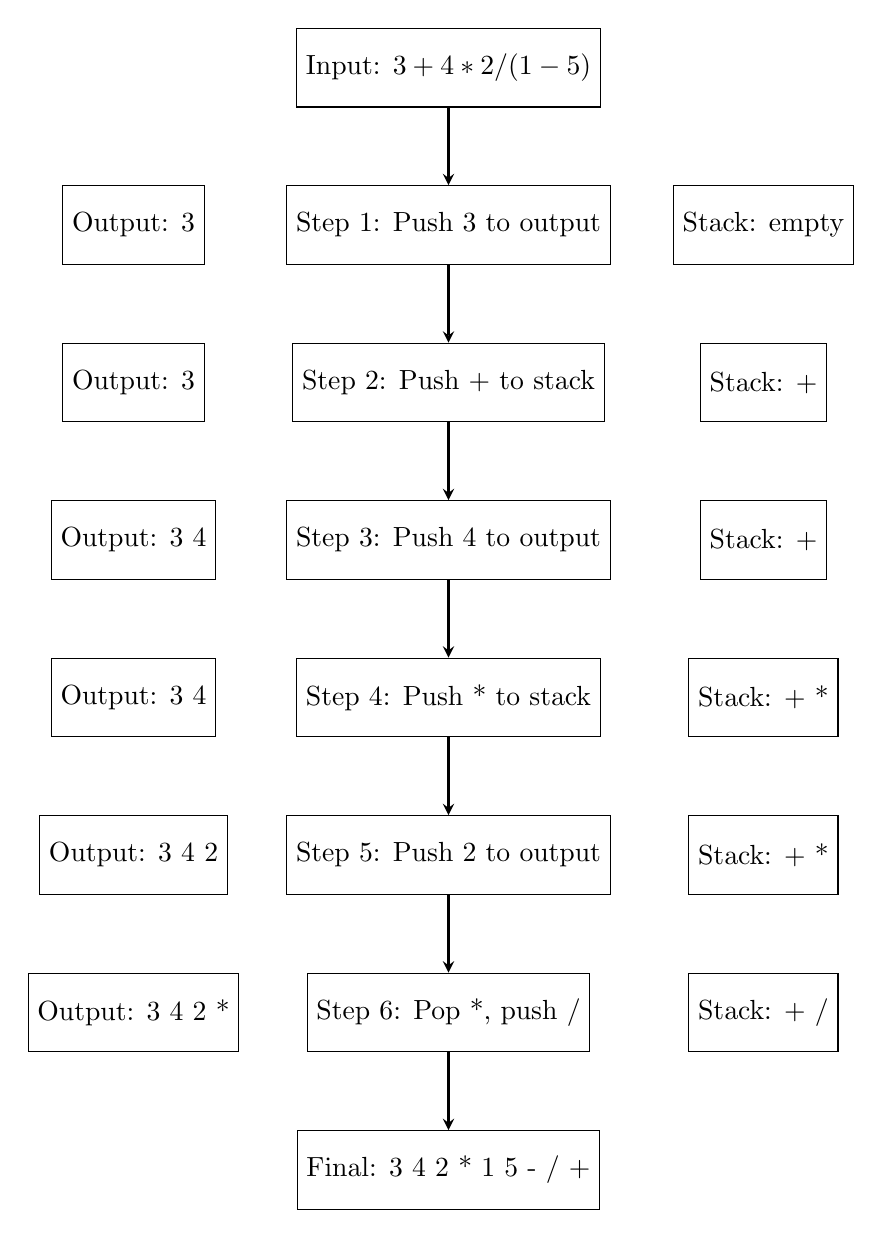
\begin{tikzpicture}[
        node distance=1cm,
        auto,
        box/.style={rectangle, draw, minimum width=1.5cm, minimum height=1cm},
        arrow/.style={->, >=stealth, thick}
    ]
    
    \node [box] (input) at (0,0) {Input: $3 + 4 * 2 / (1 - 5)$};
    
    \node [box] (step1) at (0,-2) {Step 1: Push 3 to output};
    \node [box] (stack1) at (4,-2) {Stack: empty};
    \node [box] (output1) at (-4,-2) {Output: 3};
    
    \node [box] (step2) at (0,-4) {Step 2: Push + to stack};
    \node [box] (stack2) at (4,-4) {Stack: +};
    \node [box] (output2) at (-4,-4) {Output: 3};
    
    \node [box] (step3) at (0,-6) {Step 3: Push 4 to output};
    \node [box] (stack3) at (4,-6) {Stack: +};
    \node [box] (output3) at (-4,-6) {Output: 3 4};
    
    \node [box] (step4) at (0,-8) {Step 4: Push * to stack};
    \node [box] (stack4) at (4,-8) {Stack: + *};
    \node [box] (output4) at (-4,-8) {Output: 3 4};
    
    \node [box] (step5) at (0,-10) {Step 5: Push 2 to output};
    \node [box] (stack5) at (4,-10) {Stack: + *};
    \node [box] (output5) at (-4,-10) {Output: 3 4 2};
    
    \node [box] (step6) at (0,-12) {Step 6: Pop *, push /};
    \node [box] (stack6) at (4,-12) {Stack: + /};
    \node [box] (output6) at (-4,-12) {Output: 3 4 2 *};
    
    \node [box] (final) at (0,-14) {Final: 3 4 2 * 1 5 - / +};
    
    \draw [arrow] (input) -- (step1);
    \draw [arrow] (step1) -- (step2);
    \draw [arrow] (step2) -- (step3);
    \draw [arrow] (step3) -- (step4);
    \draw [arrow] (step4) -- (step5);
    \draw [arrow] (step5) -- (step6);
    \draw [arrow] (step6) -- (final);
    
    \end{tikzpicture}
    \caption{Visual Representation of the Example}
    \label{fig:example}
\end{figure}

\section{Implementing BODMAS Rule}

The BODMAS rule (Brackets, Orders, Division, Multiplication, Addition, Subtraction) is inherently implemented in the Shunting Yard algorithm through operator precedence. The algorithm processes operations in the correct order by:

\begin{enumerate}
    \item Handling brackets by pushing left brackets onto the stack and popping operators until the matching right bracket is found
    \item Assigning higher precedence to multiplication and division than addition and subtraction
    \item Processing operators of equal precedence from left to right (for left-associative operators)[4]
\end{enumerate}

\begin{figure}[h]
    \centering
    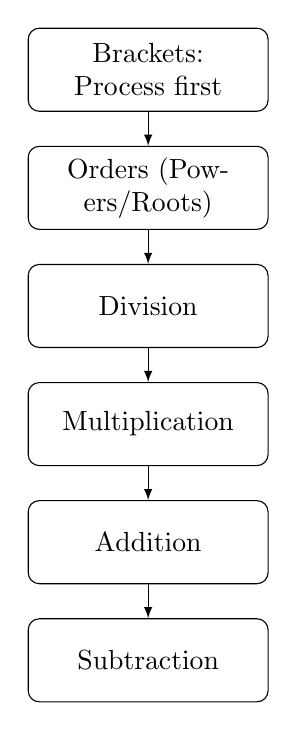
\begin{tikzpicture}[
        node distance=1.5cm,
        auto,
        block/.style={rectangle, draw, text width=8em, text centered, rounded corners, minimum height=3em},
        line/.style={draw, -latex}
    ]
    
    \node [block] (brackets) {Brackets: Process first};
    \node [block, below of=brackets] (orders) {Orders (Powers/Roots)};
    \node [block, below of=orders] (division) {Division};
    \node [block, below of=division] (multiplication) {Multiplication};
    \node [block, below of=multiplication] (addition) {Addition};
    \node [block, below of=addition] (subtraction) {Subtraction};
    
    \path [line] (brackets) -- (orders);
    \path [line] (orders) -- (division);
    \path [line] (division) -- (multiplication);
    \path [line] (multiplication) -- (addition);
    \path [line] (addition) -- (subtraction);
    
    \end{tikzpicture}
    \caption{BODMAS Rule Implementation}
    \label{fig:bodmas}
\end{figure}

\section{Function Implementation}

To implement functions like sin, cos, etc., the algorithm needs to be extended:

\begin{enumerate}
    \item When a function token is encountered, push it onto the operator stack
    \item When processing a function's arguments (which may be separated by commas), handle them appropriately
    \item When the function's closing parenthesis is encountered, pop the function from the stack to the output queue[6]
\end{enumerate}

For example, to handle $\sin(x)$ or $\max(x,y)$, the function name is pushed onto the stack when encountered, and popped to the output queue after its arguments have been processed.

\begin{figure}[h]
    \centering
    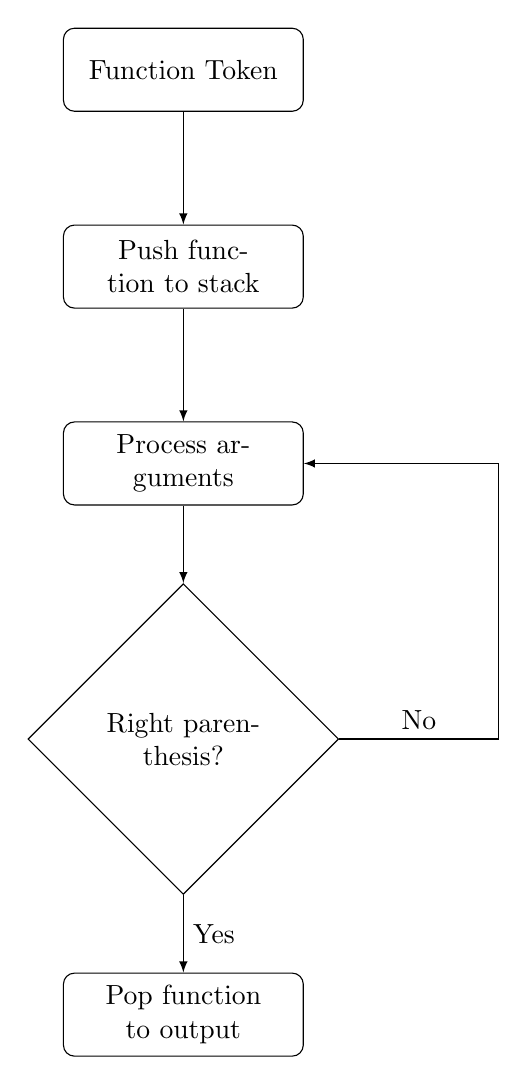
\begin{tikzpicture}[
        node distance=2cm,
        auto,
        block/.style={rectangle, draw, text width=8em, text centered, rounded corners, minimum height=3em},
        decision/.style={diamond, draw, text width=8em, text centered, minimum height=4em},
        line/.style={draw, -latex}
    ]
    
    \node [block] (start) {Function Token};
    \node [block, below of=start, node distance=2.5cm] (push) {Push function to stack};
    \node [block, below of=push, node distance=2.5cm] (args) {Process arguments};
    \node [decision, below of=args, node distance=3.5cm] (rparen) {Right parenthesis?};
    \node [block, below of=rparen, node distance=3.5cm] (pop) {Pop function to output};
    
    \path [line] (start) -- (push);
    \path [line] (push) -- (args);
    \path [line] (args) -- (rparen);
    \path [line] (rparen) -- node[right] {Yes} (pop);
    \path [line] (rparen) -- node[above] {No} ++(4,0) |- (args);
    
    \end{tikzpicture}
    \caption{Function Handling in the Shunting Yard Algorithm}
    \label{fig:function}
\end{figure}


\section{Bracket Handling}

Brackets are crucial for overriding the default operator precedence. The algorithm handles them as follows:

\begin{enumerate}
    \item When a left bracket '(' is encountered, it is pushed onto the stack
    \item When a right bracket ')' is encountered:
    \begin{itemize}
        \item Pop operators from the stack to the output queue until a left bracket is found
        \item Discard the left bracket
        \item If the token at the top of the stack is a function, pop it to the output queue
    \end{itemize}
\end{enumerate}

This ensures that expressions within brackets are evaluated first, respecting the BODMAS rule.

\section{Complexity Analysis}

The Shunting Yard algorithm has linear time complexity $O(n)$, where $n$ is the number of tokens in the input expression. Each token is processed exactly once, and each operation (push, pop) takes constant time.

\section{Evaluating Reverse Polish Notation}

After converting an infix expression to Reverse Polish Notation (RPN) using the Shunting Yard Algorithm, the next step is to evaluate the RPN expression. This process is straightforward and efficient, making RPN particularly useful for expression evaluation in computing applications.

\subsection{Understanding RPN}

RPN, also known as postfix notation, is a mathematical notation where operators follow their operands. For example, the infix expression "3 + 4" is written as "3 4 +" in RPN. This notation eliminates the need for parentheses and simplifies the evaluation process.

\subsection{Evaluation Algorithm}

The algorithm for evaluating RPN expressions uses a stack data structure and follows these steps:

\begin{enumerate}
\item Initialize an empty stack.
\item Read the RPN expression from left to right:
\begin{itemize}
\item If the token is an operand (number), push it onto the stack.
\item If the token is an operator, pop the required number of operands from the stack, perform the operation, and push the result back onto the stack.
\end{itemize}
\item After processing all tokens, the final result will be the only value remaining on the stack.
\end{enumerate}

\subsection{Example Evaluation}

Let's evaluate the RPN expression resulting from our previous example: 


\begin{equation*}
    3~4~2 * 1~5 - 2~3~\mathbin{\char`\^} \mathbin{\char`\^} ~/ ~+
\end{equation*}


\begin{table}[h]
\centering
  \begin{tabular}{ccc}
\toprule
\textbf{Token} & \textbf{Stack (after processing)} & \textbf{Explanation} \\
\midrule
3 & & Push 3 onto the stack \\
4 & & Push 4 onto the stack \\
2 & & Push 2 onto the stack \\
& & Pop 4 and 2, multiply: $4 \times 2 = 8$, push result \\
1 & & Push 1 onto the stack \\
5 & & Push 5 onto the stack \\
& $[3, 8, -4]$ & Pop 1 and 5, subtract: $1 - 5 = -4$, push result \\
2 & $[3, 8, -4, 2]$ & Push 2 onto the stack \\
3 & $[3, 8, -4, 2, 3]$ & Push 3 onto the stack \\
$\vee$ & $[3, 8, -4, 8]$ & Pop 2 and 3, exponentiate: $2^3 = 8$, push result \\
$\vee$ & $[65536]$ & Pop -4 and 8, exponentiate: $(-4)^8 = 65536$, push result \\
/ & & Pop 8 and 65536, divide: $8 / 65536 = 0$ (integer division), push result \\
=> & Pop 3 and 0, add: $3 + 0 = 3$, push result \\
\bottomrule
\end{tabular}
\caption{Step-by-step evaluation of the RPN expression}
\label{tab:rpn_evaluation}
\end{table}

Final result: 3

\subsection{Advantages of RPN Evaluation}

Evaluating RPN expressions offers several advantages:

\begin{enumerate}
\item \textbf{Simplicity}: The evaluation algorithm is straightforward and easy to implement.
\item \textbf{Efficiency}: RPN can be evaluated in a single pass from left to right, without the need for backtracking or complex parsing.
\item \textbf{No parentheses}: RPN eliminates the need for parentheses, reducing complexity and potential errors.
\item \textbf{Stack-based}: The stack-based approach aligns well with computer architecture, potentially leading to more efficient implementations.
\end{enumerate}

\section{Connecting Shunting Yard and RPN Evaluation}

The Shunting Yard Algorithm and RPN evaluation work together to provide a complete solution for parsing and evaluating mathematical expressions:

\begin{enumerate}
\item The Shunting Yard Algorithm converts infix notation to RPN, handling operator precedence and associativity.
\item The RPN evaluation algorithm then processes the resulting postfix expression to compute the final result.
\end{enumerate}

This two-step process allows for efficient and unambiguous evaluation of complex mathematical expressions, making it valuable in various applications such as calculators, compilers, and mathematical software.

\section{Conclusion}

The combination of the Shunting Yard Algorithm for infix-to-postfix conversion and the stack-based RPN evaluation method provides a robust and efficient approach to expression parsing and evaluation. This approach handles operator precedence, associativity, and nested expressions with ease, while offering a straightforward evaluation process.

By understanding and implementing these algorithms, developers can create powerful tools for mathematical expression handling, benefiting applications in fields such as computer algebra systems, calculators, and programming language design.

 
\end{document}
